\section{Experimental Setup}
\label{sec:exp}

We design two experiments, one for evaluating different similarity measures, and the other one for the sentence alignment. The datasets and metrics used are introduced below.

\subsection{Similarity Measure}

The similarity measure is evaluated based on a paraphrase detection task performed on Microsoft Research Paraphrase Corpus (MSRC), SICK, and Modern/Original Version of Shakespeare scripts. For unsupervised similarity measure, the three sentence embedding schemes with multiple embedding dimensions for word embeddings are combined with the two distance measures, and together with a set of thresholds, are used to label sentences with a similarity score above threshold as paraphrases. We also used BLEU~\cite{papineni2002bleu} and ROUGE~\cite{lin2004rouge}, as baseline models in this task.

\subsection{Sentence Alignment}

The datasets on sentence alignment are a part of the final documents that are aligned, including \emph{Anna Karenina}, \emph{The Story of Stone} and \emph{The Brothers Karamazov}. Related data for each corpus is shown in Table \ref{tb:1}.

\begin{table}[h!]\footnotesize
	\centering
	\small
	\begin{tabular}{|c|c|c|}
		\hline
		Corpus & Translation 1 & Translation 2 \\
		\hline
		Anna Karenina & 21,398 & 20,973 \\
		The Story of Stone & 46,034 & 56,256 \\
		The Brothers Karamazov & 24,133 & 20,288 \\
		\hline
	\end{tabular}
	\caption{Size of Datasets (Number of Words).}\label{tb:1}
\end{table}

The evaluation of sentence alignment is based on the following considerations.
\begin{enumerate}
	\item \emph{Efficiency.} The time a model takes to align sentences should be reasonable with respect to the number of sentences in the raw documents.
	\item \emph{Percentage of aligned sentences.} Although the main focus of this research is to construct a corpus with high quality, the percentage of aligned sentences should also be considered. Namely, we want to assess how many sentences should be aligned are actually aligned by the model.
	\item \emph{Quality.} Since it is hard to assess whether all sentences are properly aligned or not, we sample a fraction of aligned sentences and decide whether each pair should be aligned manually. The quality of the alignment is evaluated as the percentage of the pairs that are ``properly aligned'' with respect to the number of total aligned pairs. The level of properness for a aligned pair is defined as follows, based on Huang's criteria~\cite{hwang2015aligning}.
	\begin{itemize}
		\item \textbf{Good}: 
		\begin{enumerate}
			\item completely the same;
			\item possibly some word substitutions and structural modifications;
			\item describe the same object, environment, or situation using different but the same type of adjectives, nouns, sentiments, etc.;
			\item convey the same type of sentiments in short conversations.
		\end{enumerate}
		\item \textbf{Good Partial}:
		\begin{enumerate}
			\item one sentence is good aligned with respect to a part of the other sentence;
			\item the sentence contains some additional clauses or phrases that have information which is not contained within the other sentence;
		\end{enumerate}
		\item \textbf{Partial}:
		\begin{enumerate}
			\item a part of a sentence is good aligned with respect to a part of the other sentence;
			\item both sentences contain some additional clauses or phrases that have information which is not contained within the other;
		\end{enumerate}
		\item \textbf{Bad}: the sentences discuss unrelated contents.
	\end{itemize}
	From above, the first three categories are considered as ``properly aligned''. The definition is relatively loose for stylized expressions. It happens that in an aligned sentence pair, one contains additional expressions than the other. But the main content of the pair should be consistent.
\end{enumerate}

For the following discussion, the ``percentage'' represents the portion of sentences that are aligned in the raw documents, and the ``quality'' represents the portion of aligned pairs that are proper.

\section{Results}
\label{sec:results}

Experimental results for similarity measure and sentence alignment are presented in the next two sections. It is shown that the unsupervised similarity measure is comparable with supervised similarity measures, and that we have a relatively strong similarity scoring system for sentence alignment. Then we verify that our sentence alignment model is superior to the baseline model in terms of robustness and quality.

\subsection{Similarity Measure}
The result for MSRC with different thresholds is shown in Figure \ref{fig:5}. From the figure we can observe that the highest accuracy is reached by ``WDV + MAX + COS'' at threshold around 0.7, with the second highest accuracy reached by the ``UNV + COS'' combination. 

\begin{figure}[htbp]
	\centering
	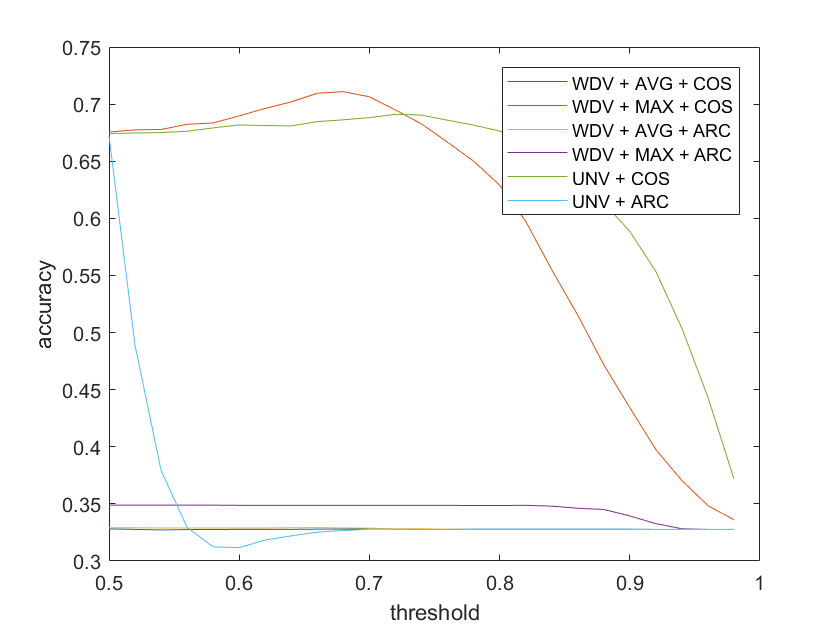
\includegraphics[width=8cm]{./5.png}
	\caption{Accuracies for MSRC with Different Threshold $t$.}\label{fig:5}
\end{figure}

One observation is that the cosine measurement is superior to the arccos measurement, which is the case also for SICK and Shakespeare (SHPR). This might be an indication that cosine measure is a more reasonable measure for spatial distance in the vector space of sentence embeddings.

For each experimented similarity measurement method, the best dimension for word embedding and the best threshold is used for the final comparison. The dimension is fixed as 100. The results for both supervised and unsupervised methods are shown in Table \ref{tb:2}. (INF-F and INF-G are InferSent models using GloVe and fasttext pretrained word vectors, respectively.)

\begin{table}[h!]\footnotesize
	\centering
	\small
	\begin{tabular}{|c|c|c|c|}
		\hline
		\diagbox{Method}{Accuracy (\%)}{Corpus} & MSRC & SICK & SHPR \\
		\hline
		\hline
		WDV + AVG + COS & 32.8 & 36.6 & 52.5 \\
		WDV + MAX + COS & 71.1 & 68.1 & 72.0 \\
		WDV + AVG + ARC & 32.9 & 36.7 & 53.9 \\
		WDV + MAX + ARC & 34.9 & 39.4 & 54.7 \\
		UNV + COS & 67.9 & \textbf{74.2} & 77.6 \\
		UNV + ARC & 67.2 & 63.5 & 50.0 \\
		INF-F + COS & \textbf{72.2} & 72.5 & \textbf{78.6} \\
		INF-F + ARC & 67.2 & 63.5 & 50.6 \\
		INF-G + COS & 70.4 & 73.0 & 73.9 \\
		INF-G + ARC & 67.2 & 63.4 & 50.8 \\
		\hline
		MaLSTM & 56.9 & 78.3 & 71.6 \\
		TF-KLD & 70.8 & 74.5 & 86.1 \\
		\hline
		BLEU & 69.9 & 65.9 & 71.0 \\
		ROUGE & 71.3 & 67.8 & 71.8 \\
		\hline
	\end{tabular}
	\caption{Paraphrase Detection Accuracies.}\label{tb:2}
\end{table}

From the results, we can conclude that the similarity measurement ability on both standard paraphrase corpus and literature corpus is competent compared with state-of-art similarity models, and especially, supervised models. In the sentence alignment task, the ability to measure sentence similarity and the efficiency of this evaluation should both be considered, since the documents to be aligned might be so large that the sentence encoding model costs a lot of computing resources.

\subsection{Sentence Alignment}

Table \ref{tb:7} shows how filter mechanism affects the alignment quantity and quality\footnote{The model names are abbreviated as ``model + filter'' schemes. For instance, ``BLEU + UNV'' means BLEU model for the first three stages of alignment, and Universal Sentence Encoder model for the last stage of filtering.}. The results verify that our filter scheme does largely improve the overall performances of alignment models. Specifically, ``BLEU + UNV'' and ``WDV + UNV'' combinations outperform other models in both quality and quantity, these two combinations will be used for end-to-end comparison.

\begin{table*}[htbp]\footnotesize
	\centering
	\small
	\begin{tabular}{|c|c|c|c|c|c|c|c|c|c|c|}
		\hline
		\textbf{\diagbox{Result}{Model}} & \textbf{BLEU} & \textbf{INF} & \textbf{WDV} & \textbf{UNV} & \textbf{\tabincell{c}{BLEU \\ + \\ UNV}} & \textbf{\tabincell{c}{BLEU \\ + \\ INF}} & \textbf{\tabincell{c}{WDV \\+ \\ UNV }} & \textbf{\tabincell{c}{WDV \\ + \\ INF }} & \textbf{\tabincell{c}{INF \\ + \\ UNV }} & \textbf{\tabincell{c}{UNV \\ + \\ INF }}  \\
		\hline
		\hline
		Time & 1.9m & 8.4m & 4.5m & 1.7h & 10.8m & 9.8m & 19.4m & 8.1m & 24.8m & 3.6h \\
		Percentage [\%] & 73.7 & 70.9 & 73.7 & 42.2 & 87.1 & 85.0 & 85.6 & 85.2 & 17.7 & 53.6  \\
		Quality [\%] & 100 & 98 & 98 & 91 & 100 & 100 & 98 & 97 & 100 & 99 \\
		\hline
	\end{tabular}
	\caption{Quantitative Results (\emph{Notre Dame de Paris}).}\label{tb:7}
\end{table*}

We perform our alignment model on other three pairs of documents, \emph{Anna Karenina}, \emph{The Story of Stone}, and \emph{The Brothers Karamazov}. The results are shown in Table \ref{tb:8}.

\begin{table*}[htbp]\footnotesize
	\centering
	\small
	\begin{tabular}{|c|c|c|c|c|c|c|c|}
		\hline
		\textbf{\diagbox{Model}{Result}} & Time & Percentage [\%] & G [\%] & GP [\%] & P [\%] & B [\%] & Quality [\%] \\
		\hline
		\multicolumn{8}{|c|}{Anna Karenina} \\
		\hline
		This work & 0.78h & \textbf{68.7} & 90 & 5 & 3 & 2 & \textbf{98} \\
		Bleualign & 23.44s & 37.2 & 53 & 19 & 5 & 23 & 77 \\
		\hline
		\multicolumn{8}{|c|}{The Story of Stone} \\
		\hline
		This work & 8.2h & 19.2 & 35 & 29 & 16 & 20 & \textbf{80} \\
		Bleualign & 51.56s & 25.5 & 10 & 11 & 19 & 60 & 40 \\
		\hline
		\multicolumn{8}{|c|}{The Brothers Karamazov} \\
		\hline
		This work & 1.1h & \textbf{53.2} & 67 & 24 & 7 & 2 & \textbf{98} \\
		Bleualign & 24.33s & 33.0 & 32 & 38 & 9 & 21 & 79 \\
		\hline
	\end{tabular}
	\caption{Quantitative Results ([1] \emph{Notre Dame de Paris}, [2] \emph{The Story of Stone}).}\label{tb:8}
\end{table*}

Although the baseline model, Bleualign performs the fastest among the compared schemes, it does not guarantee the quality of aligned sentences. Moreover, since it highly relies on word alignment, it fails in aligning comparable documents that are not so much alike at the first glance, such as \emph{The Story of Stone}. The following shows a sample pair which is misaligned by the Bleualign model, but is properly aligned by our method.

\textbf{Sentence}: \emph{His second child was a daughter, born strangely enough on the first day of the year.}

\textbf{Bleualign}: \emph{The first qin emperor,}

\textbf{Our model}: \emph{The second child she bore him was a little girl, rather remarkable because she was born on new year’s day.}

As a qualitative analysis on model misbehaviors, we take a few representative sentences from the results that are not properly aligned by different models in the experiment, as is in Table \ref{tb:4}. 

One can notice that word-based alignment schemes, such as BLEU, WDV, and the Bleualign model, is not competent in handling short sentences, while sentence-based alignment schemes fail in cases of longer sentences. This can serve as an argument for using similarity measurements from both perspectives, as a compensation for each other. Furthermore, word-level similarity measures can serve as better anchors in the first stage of our model, and sentence-level similarity measures serve well as filters in the second stage, since sentence level encoders normally takes longer time to embed sentences in every single run.

\begin{table*}[h!]\footnotesize
	\centering
	\small
	\begin{tabular}{|c|c|}
		\hline
		\textbf{Model} & \textbf{Misaligned Sentence (False Positive [FP] or False Negative [FN])}  \\
		\hline
		\hline
		Bleualign [FP] & \tabincell{c}{\emph{baoyu clapped his hands in approval.} \\ \emph{you're getting quite a temper lately, master bao.}}  \\
		\hline
		BLEU [FN] & \tabincell{c}{\emph{xiang-yan and bao-chai were present that day, it was true; but the absence of...to burst into tears.} \\ \emph{seeing xiangyun and baochai there but not...wanted to take off some clothes.}}  \\
		\hline
		INF [FP] & \tabincell{c}{\emph{the priest whom the girls had noticed...was indeed archdeacon claude frollo.} (31 words) \\ \emph{but she has three things...hands by squeezing her waist.} (79 words)}  \\
		\hline
		WDV [FP] & \tabincell{c}{\emph{what's at stake here are the women.} \\ \emph{are there women or are there not?}} \\
		\hline
		UNV [FP] & \tabincell{c}{\emph{the mob repeated with a frenzied cheer.} \\ \emph{and among the monsters thus...in front of a candle.} (48 words)}  \\
		\hline
	\end{tabular}
	\caption{Aligned Corpora.}\label{tb:4}
\end{table*}

\section{Constructing a Monolingual Parallel Corpus}\label{sec:data}

We then proceed to construct a monolingual parallel corpus using the sentence alignment model. The corpus mainly comes from different versions of translation of 10 literature works. A complete list of information about the aligned works is shown Table \ref{tb:6}\footnote{The corpus might be further improved afterwards. It will be released to the research community via \url{http://anonymized.for.blind.review}.}.

To evaluate the quality of the alignment, a sample batch of sentences are selected and manually decided on whether the alignment is reasonable based on the criteria described above. The quality of the parallel corpus is represented by the percentage of ``true positive'' with respect to the total number of aligned pairs. Our work achieves reasonable alignment efficiency and generates high quality sentences for text rewriting rules.

\begin{table*}[h!]\footnotesize
	\centering
	\small
	\begin{tabular}{|c|c|c|c|c|c|}
		\hline
		\textbf{\diagbox{Corpus}{Information}} & \textbf{Author} & \textbf{Translator} & \textbf{Length} & \textbf{Aligned (\%)} & \textbf{Quality (\%)} \\
		\hline
		\hline
		\multirow{2}{*}{Notre Dame de Paris} & \multirow{2}{*}{Victor Hugo} & Alban Krailsheimer & 10272 & 86.3 & \multirow{2}{*}{99.4} \\
		\cline{3-5} 
		& & I. F. Hapgood & 10179 & 87.0 & \\
		\hline
		\multirow{2}{*}{Les Miserables} & \multirow{2}{*}{Victor Hugo} & Julie Rose & 34145 & 76.4 & \multirow{2}{*}{99.0} \\
		\cline{3-5}
		& & I. F. Hapgood & 34328 & 76.0 & \\
		\hline
		\multirow{2}{*}{The Story of Stone} & \multirow{2}{*}{Cao Xueqin} & Yang Xianyi & 46034 & 9.7 & \multirow{2}{*}{94.0} \\
		\cline{3-5}
		& & David Hawkes & 56256 & 8.6 &  \\
		\hline
		\multirow{2}{*}{The Brothers Karamazov} & \multirow{2}{*}{F. Dostoevsky} & A. R. MacAndrew & 24133 & 58.6 & \multirow{2}{*}{95.3} \\
		\cline{3-5}
		& & Richard Pevear & 20288 & 68.1 & \\
		\hline
		\multirow{2}{*}{Crime and Punishment} & \multirow{2}{*}{F. Dostoevsky} & Michael R. Katz & 14503 & 70.6 & \multirow{2}{*}{93.9} \\
		\cline{3-5}
		& & Richard Pevear & 12938 & 76.2 & \\
		\hline
		\multirow{2}{*}{The Magic Mountain} & \multirow{2}{*}{Thomas Mann} & John E. Woods & 14464 & 83.8 & \multirow{2}{*}{97.6} \\
		\cline{3-5}
		& & H. T. Lowe-Porter & 14231 & 83.8 & \\
		\hline
		\multirow{2}{*}{The Illiad} & \multirow{2}{*}{Homer} & Ian C. Johnston & 7744 & 68.1 & \multirow{2}{*}{72.5} \\
		\cline{3-5}
		& & Robert Fagles & 7237 & 58.5 & \\
		\hline
		\multirow{2}{*}{Don Quixote} & \multirow{2}{*}{Cervantes Saavedra} & John Rutherford & 11902 & 48.5 & \multirow{2}{*}{84.4} \\
		\cline{3-5}
		& & John Ormsby & 9056 & 58.3 & \\
		\hline
		\multirow{2}{*}{Anna Karenina} & \multirow{2}{*}{Leo Tolstoy} & Pevear and Volokhonsky & 21398 & 74.6 & \multirow{2}{*}{99.3} \\
		\cline{3-5}
		& & Rosamund Bartlett & 20971 & 74.5 & \\
		\hline
		\multirow{2}{*}{Madame Bovary} & \multirow{2}{*}{Gustave Flaubert} & Eleanor Marx-Aveling & 6670 & 73.9 & \multirow{2}{*}{97.6} \\
		\cline{3-5}
		& & Margaret Mauldon & 6837 & 72.8 & \\
		\hline
	\end{tabular}
	\caption{Aligned Corpora.}\label{tb:6}
\end{table*}

In order to guarantee the quality of the corpus, the percentage of aligned sentences with respect to the original length is not necessarily maximized. Besides, some aligned pairs contain sentences that are exactly identical. We did not discard them, since in order to learn monolingual text rewriting rules, the mappings of some expressions to themselves is also included in the style parameter. However, for training or evaluating semantic similarity models, those sentences might be ignored.




